\documentclass{standalone}
%
\usepackage{tikz}
\usetikzlibrary{backgrounds,shapes.callouts}
\usepackage{tkz-euclide}
\usepackage{xcolor}
\usepackage{ifthen}
%
\definecolor{space}{HTML}{1F2C4E}
\definecolor{earth}{HTML}{0089FA}
\definecolor{dida}{HTML}{FFDE00}
\definecolor{title}{HTML}{FBA706}
\definecolor{moon}{HTML}{AFAFAF}
%
\usepackage{fontspec}
\setmainfont{Open Dyslexic}
%
\title{Il mondo prima}
\begin{document}
	\tikzset{
		partial ellipse/.style args = {#1:#2:#3}{insert path={+ (#1:#3) arc (#1:#2:#3)}},
		notice/.style  = { draw, ellipse callout, callout relative pointer={#1} },
	}
	\begin{tikzpicture}[background rectangle/.style={fill=white},show background rectangle,>={[inset=0,angle'=27]Stealth}]
		%title
		\draw [black,ultra thick] (1,1) rectangle (29,-1);
		\node at (15,0) {\textcolor{black}{\fontsize{40}{41}\selectfont Il mondo prima}};
		% 
		\begin{scope}[shift={(0,-23)}]
			\node at (15,0) {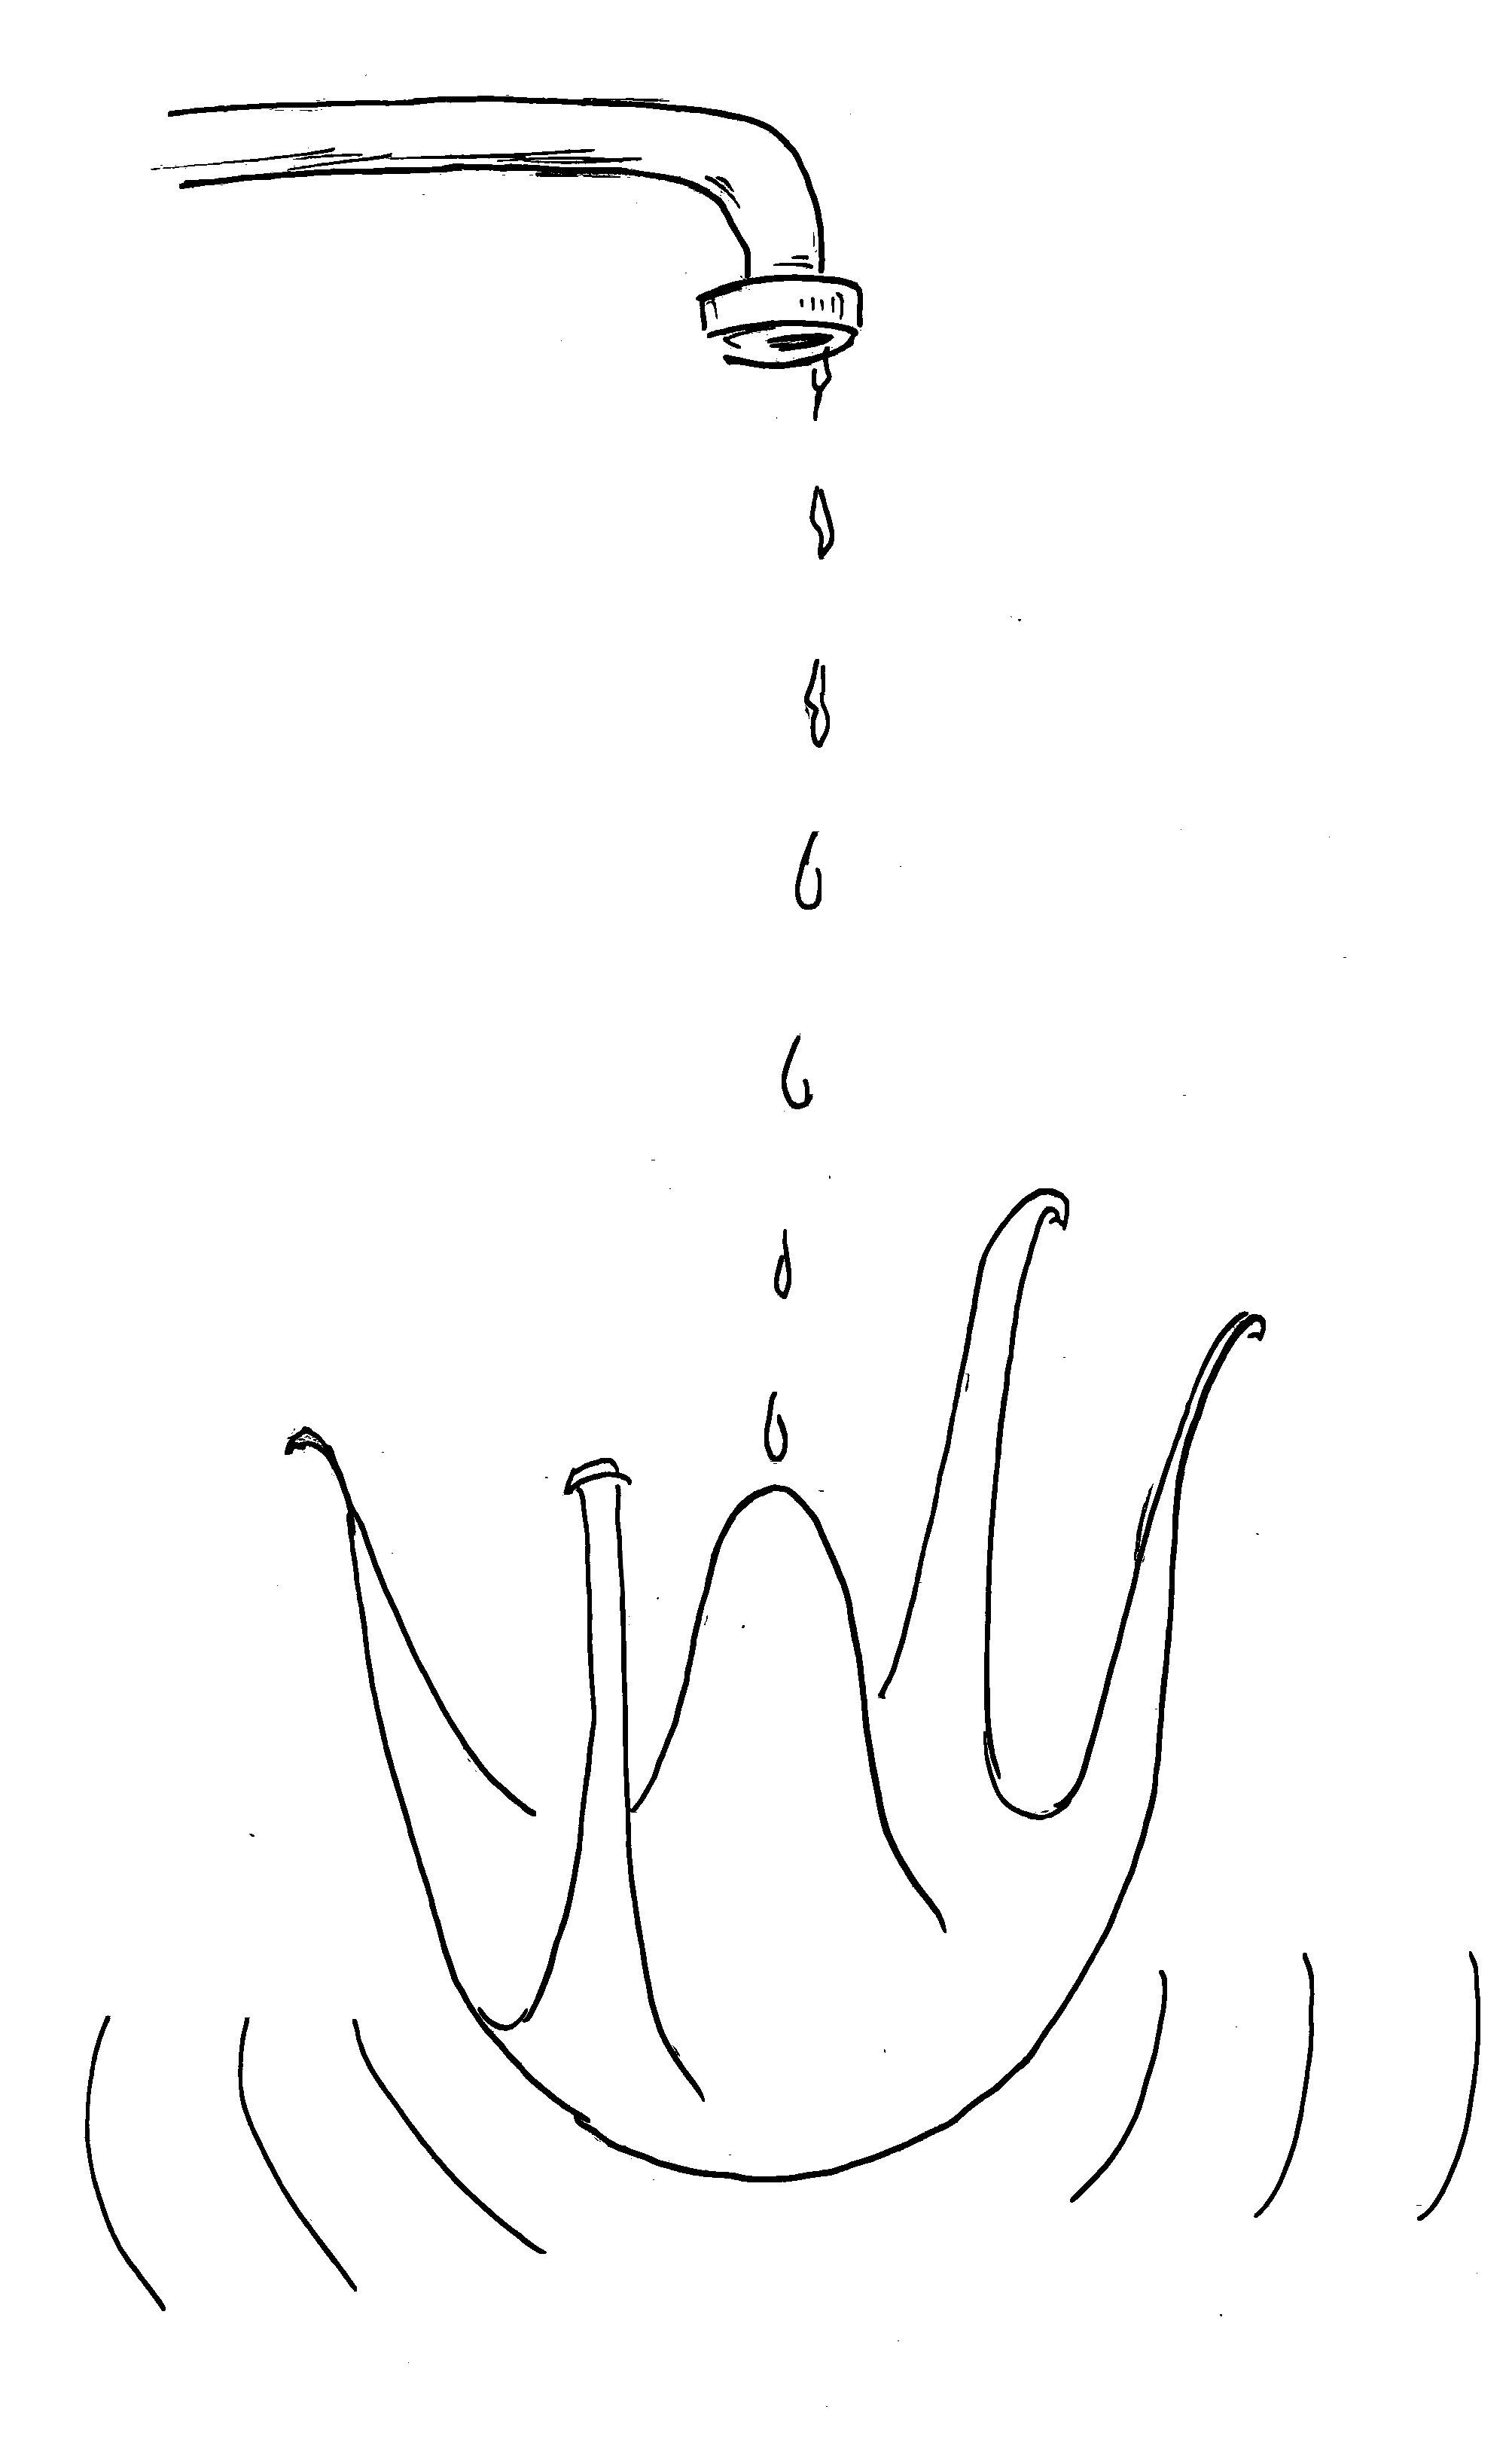
\includegraphics[width=25cm]{img-higgs/meccanismo_higgs}};
			\node (example-textwidth-2) [right, align=right, text width=10cm, color=black, font=\fontsize{18pt}{19pt}\selectfont] at (1,10) {Bosoni};
			\node (example-textwidth-2) [right, align=right, text width=10cm, color=black, font=\fontsize{18pt}{19pt}\selectfont] at (1,6) {Quark};
			\node (example-textwidth-2) [right, align=right, text width=10cm, color=black, font=\fontsize{18pt}{19pt}\selectfont] at (1,2) {Leptoni};
			% prima
			\node (example-textwidth-2) [right, align=right, text width=7cm, color=black, font=\fontsize{18pt}{19pt}\selectfont] at (7,10) {Z -> 0\\W -> 0\\g -> 0\\$\gamma$ -> 0};
			\node (example-textwidth-2) [right, align=right, text width=7cm, color=black, font=\fontsize{18pt}{19pt}\selectfont] at (7,6) {u -> 0\\d -> 0\\c -> 0\\s -> 0\\t -> 0\\b -> 0};
			\node (example-textwidth-2) [right, align=right, text width=7cm, color=black, font=\fontsize{18pt}{19pt}\selectfont] at (7,2) {e -> 0\\$\mu$ -> 0\\$\tau$ -> 0};
			% dopo
			\node (example-textwidth-2) [right, align=left, text width=7cm, color=black, font=\fontsize{18pt}{19pt}\selectfont] at (17,10) {Z -> 91.19 GeV/$c^2$\\W -> 80.36 GeV/$c^2$\\g -> 0\\$\gamma$ -> 0};
			\node (example-textwidth-2) [right, align=left, text width=7cm, color=black, font=\fontsize{18pt}{19pt}\selectfont] at (17,6) {u -> 2.2 MeV/$c^2$\\d -> 4.7 MeV/$c^2$\\c -> 1.28 GeV/$c^2$\\s -> 96 MeV/$c^2$\\t -> 173.1 GeV/$c^2$\\b -> 4.18 GeV/$c^2$};
			\node (example-textwidth-2) [right, align=left, text width=7cm, color=black, font=\fontsize{18pt}{19pt}\selectfont] at (17,2) {e -> 0.511 MeV/$c^2$\\$\mu$ -> 105.66 MeV/$c^2$\\$\tau$ -> 1.78 GeV/$c^2$};
		\end{scope}
		%
		\begin{scope}[shift={(0,-45)}]
			\node (example-textwidth-2) [right, align=left, text width=22cm, color=black, font=\fontsize{18pt}{19pt}\selectfont] at (6,0) {Era bello sapere che il tempo non contava nulla\\Era bello viaggiare leggeri per l'universo\\Il mondo prima che arrivassi te};
		\end{scope}
		% 
		\begin{scope}[shift={(0,-58)}]
			\node at (15,0) {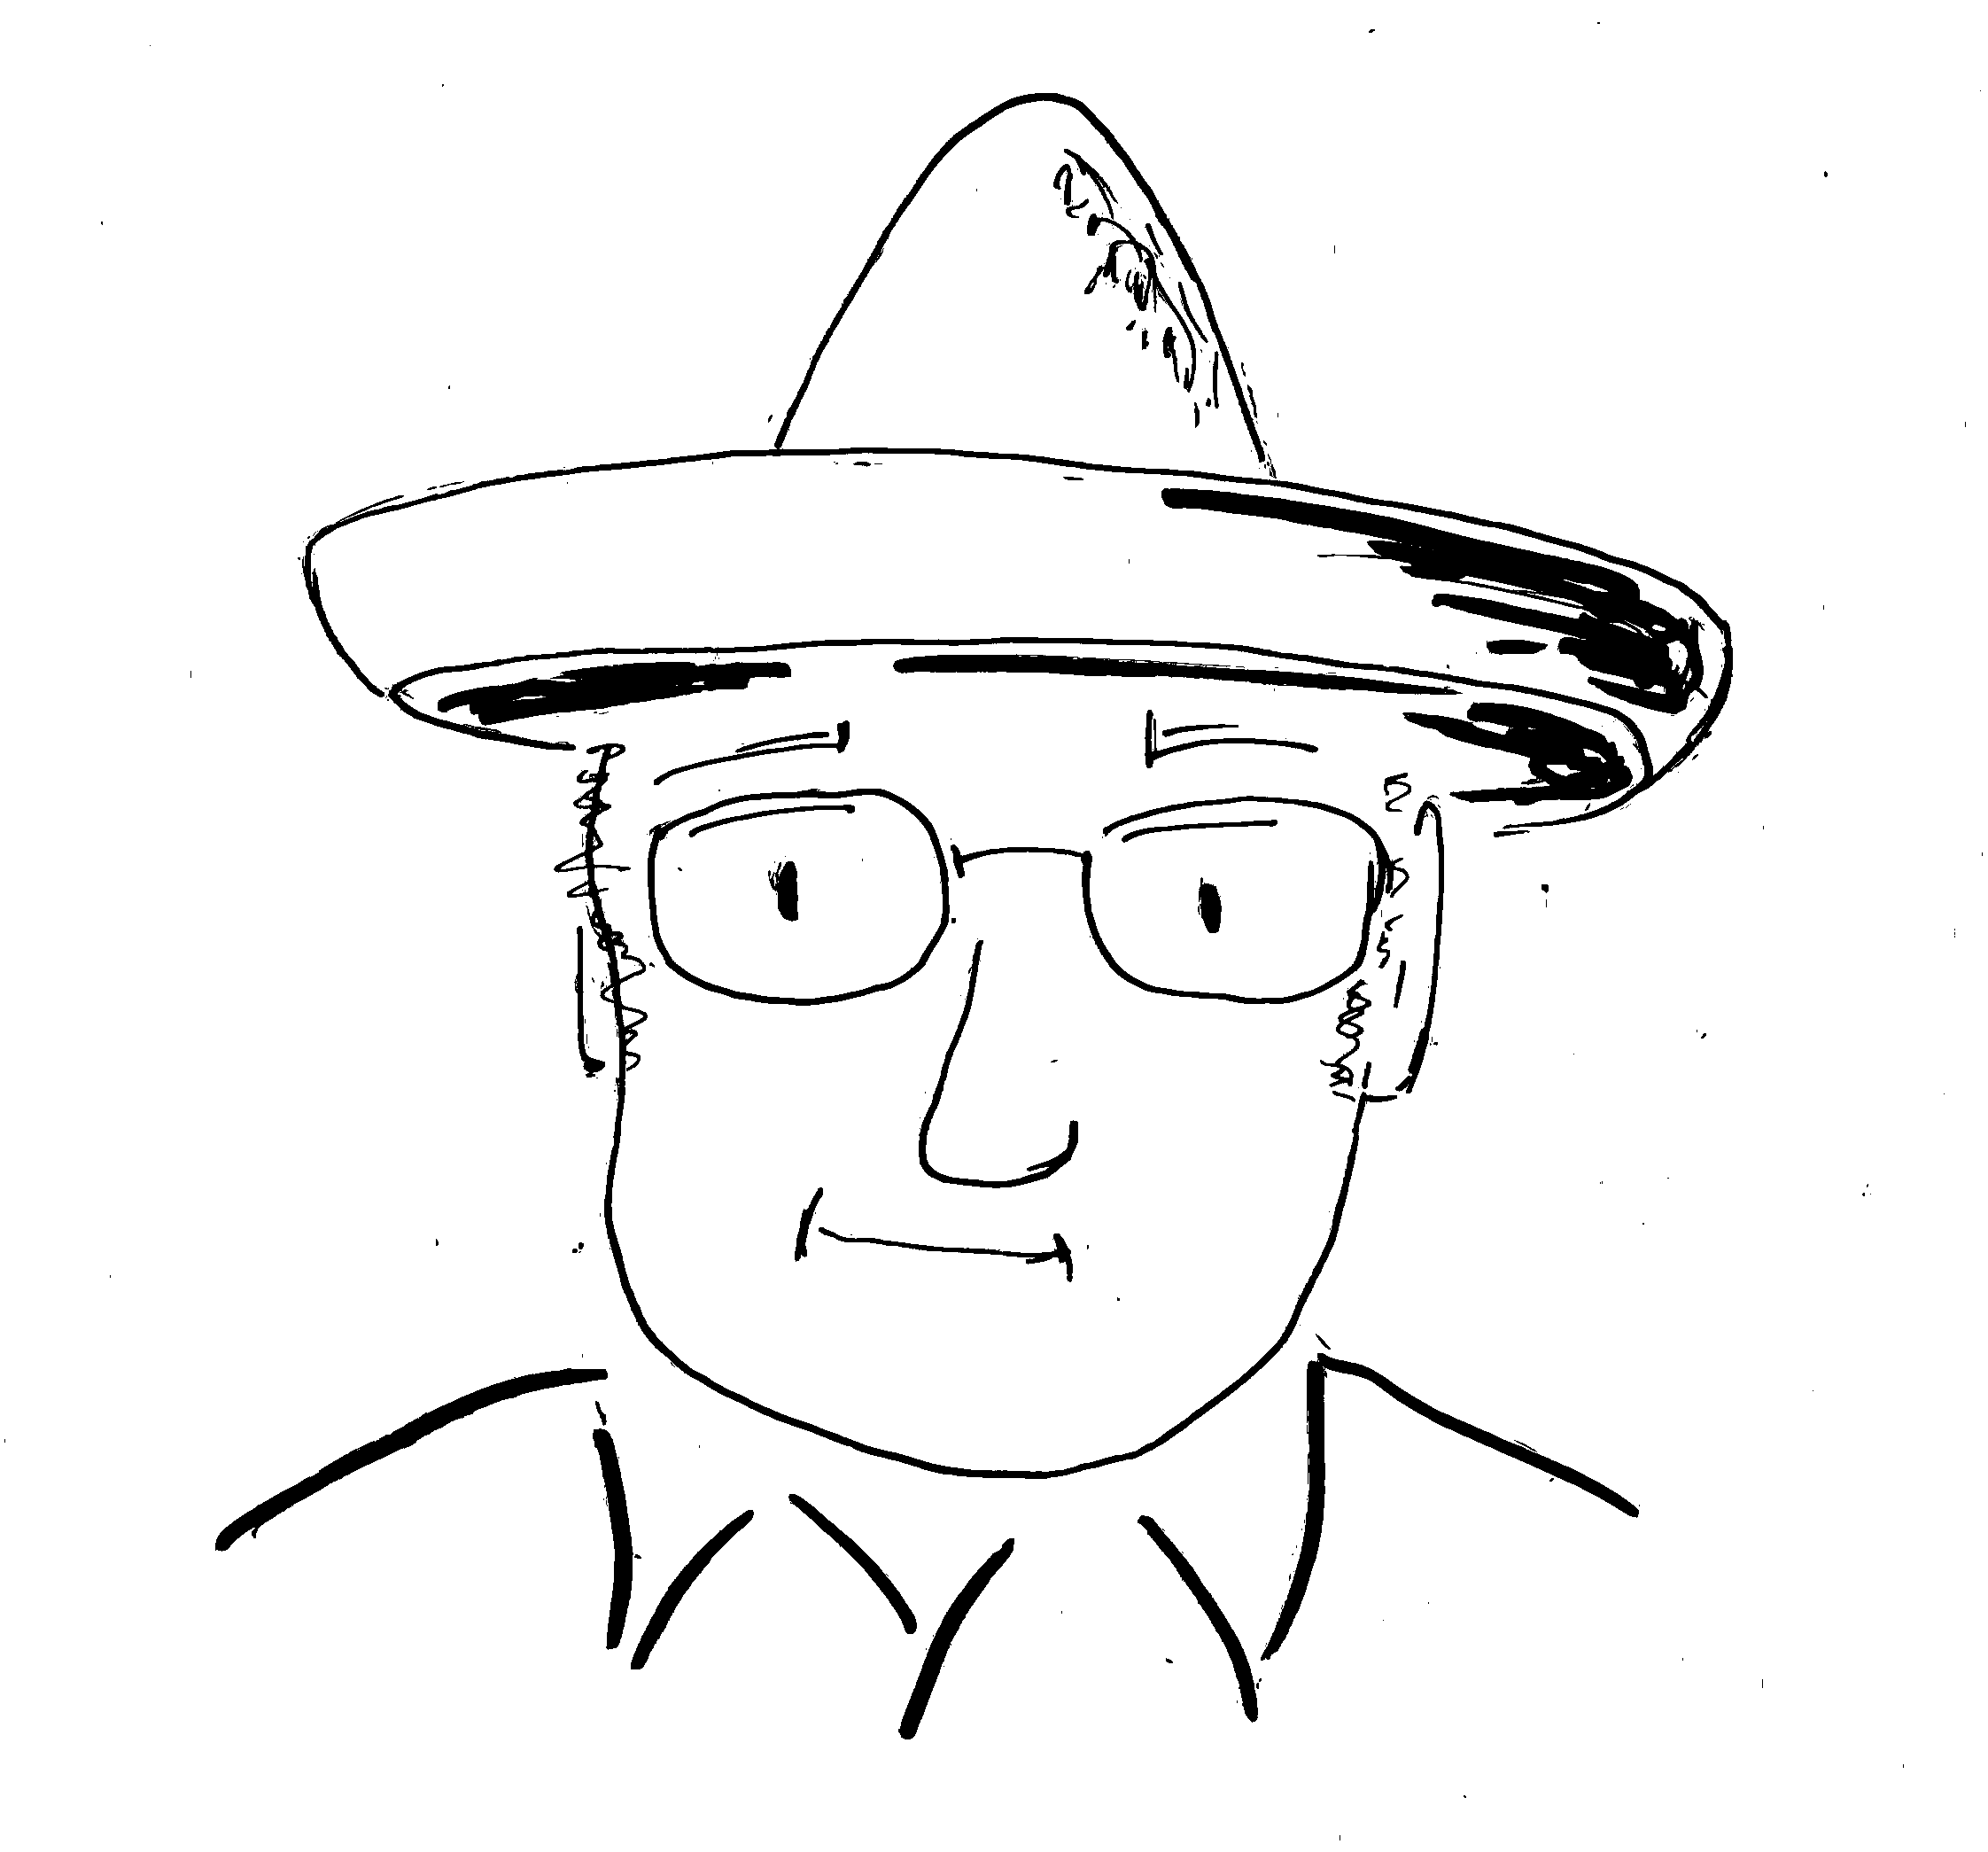
\includegraphics[width=25cm]{img-higgs/peter_higgs}};
		\end{scope}
		%
		\begin{scope}[shift={(0,-70)}]
			\draw[color=black,fill=white,ultra thick] (1,2) rectangle (29,-2);
			\node at (3,0) {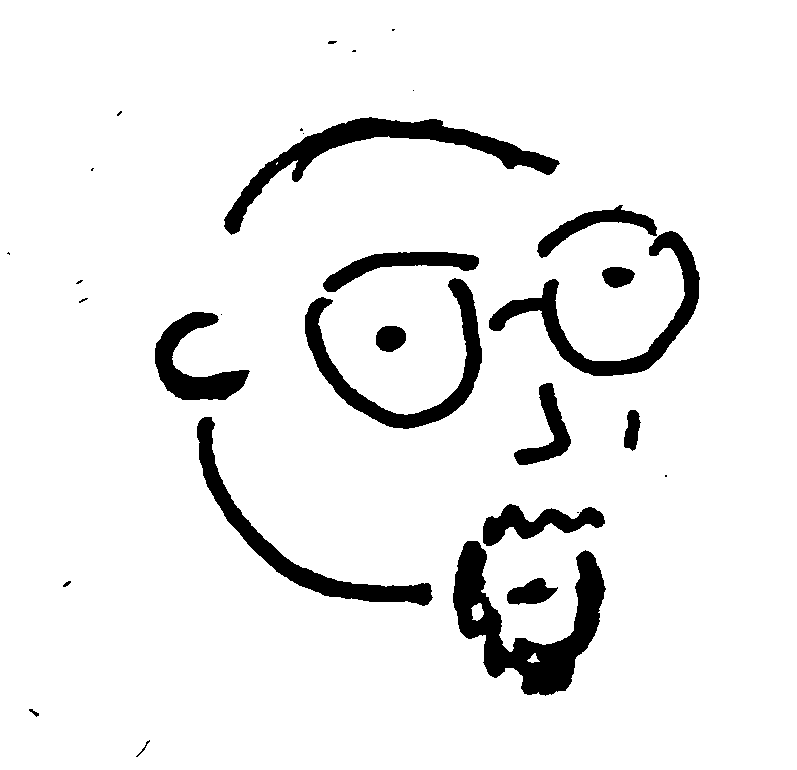
\includegraphics[width=5cm]{img-timeline/io_sx}};
			\node (example-textwidth-2) [right, align=left, text width=22cm, color=black, font=\fontsize{18pt}{19pt}\selectfont] at (6,0) {E' stato \textbf{Peter Higgs} a scoprire che al meccanismo che fornisce la massa alle particelle e' associato un bosone, il bosone che porta il suo nome, la cui massa e' pari a circa 125.11 GeV/$c^2$.};
		\end{scope}
		%
		\begin{scope}[shift={(0,-75)}]
			\node at (27,0) () {
\includegraphics[width=3.7cm]{licenza}};
			\node at (18,-0.1) {\textcolor{black}{\fontsize{14}{15}\selectfont Testo e illustrazioni: @ulaulaman - Gianluigi Filippelli}};
		\end{scope}
	\end{tikzpicture}
%
\end{document}
